\subsection*{Descomposición espectral para gas en un tubo}

\item
\begin{minipage}[t][1.6cm]{0.65\textwidth}
Un tubo contiene dos secciones de gas en reposo separadas por un tabique.
Antes de que se lo quite en $t=0$ de un lado la densidad era $\rho_{0}-\Delta$ y del otro $\rho_{0}+\Delta$ (considere $\Delta\ll\rho_{0}$).
Datos: $\rho_{0}$, $\Delta$, $L$, $v_\text{sonido}$.
\end{minipage}
\begin{minipage}[c][2cm][t]{0.3\textwidth}
	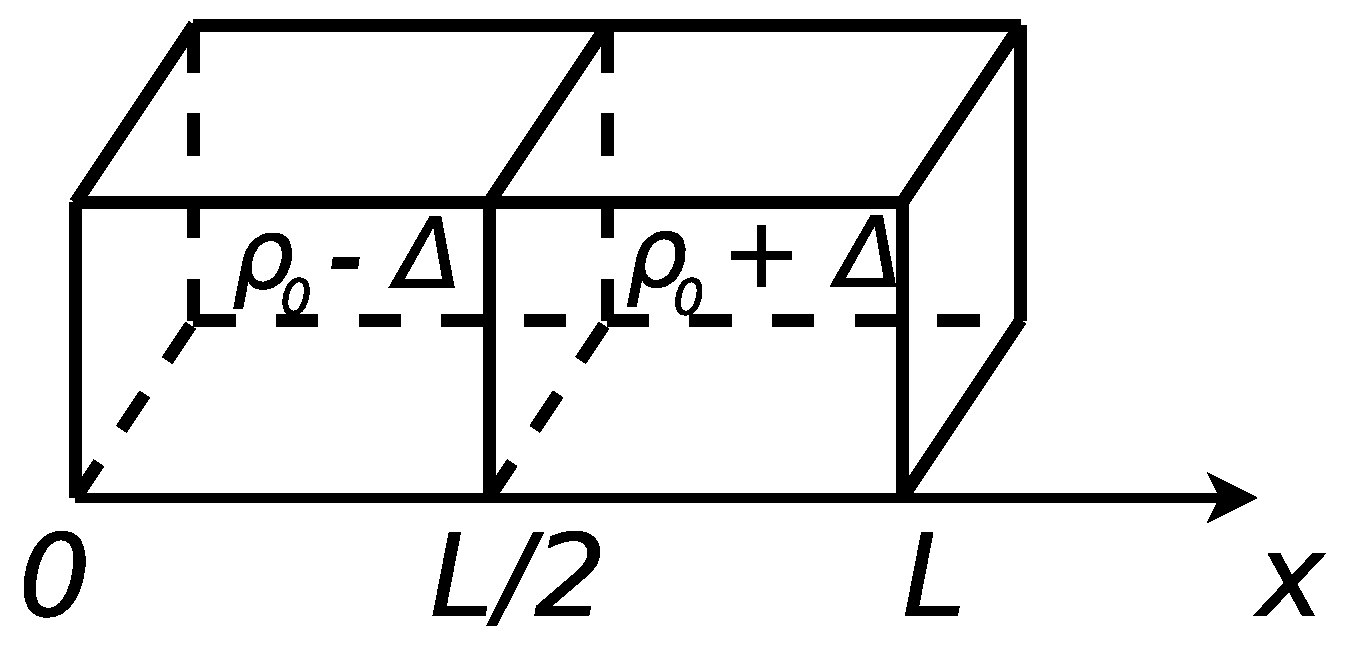
\includegraphics[width=\textwidth]{ej1-30}
\end{minipage}
\begin{enumerate}
	\item Imponga condiciones de contorno al desplazamiento de moléculas $\psi$.
	A partir de estas obtenga la expresión para un modo normal $\psi_{n}(x,t)$.
	¿Cuáles son las longitudes de onda permitidas?
	\item Halle $\psi(x,0)$ a partir de los datos sobre $\rho(x,0)$.
	\item Calcule $\psi(x,t)$ y $\rho(x,t)$.
\end{enumerate}


\item
\begin{minipage}[t][2cm]{0.65\textwidth}
Un tabique divide un tubo dividido en dos regiones.
En la izquierda hay una presión constante $p = p_0 + \Delta p$ en tanto que en la derecha está a $p_0$ pues está abierta a la atmósfera.
A $t = 0$ se remueve el tabique.

Halle $\delta p(x,t)$, $\psi(x,t)$ y $\delta\rho(x,t)$ conociendo $p_0$, $\Delta p\ll p_0$, $L$, $v_\text{sonido}$ y que $\gamma= \frac{7}{5}$ para un gas diatómico.
\end{minipage}
\begin{minipage}[c][0.6cm][t]{0.3\textwidth}
	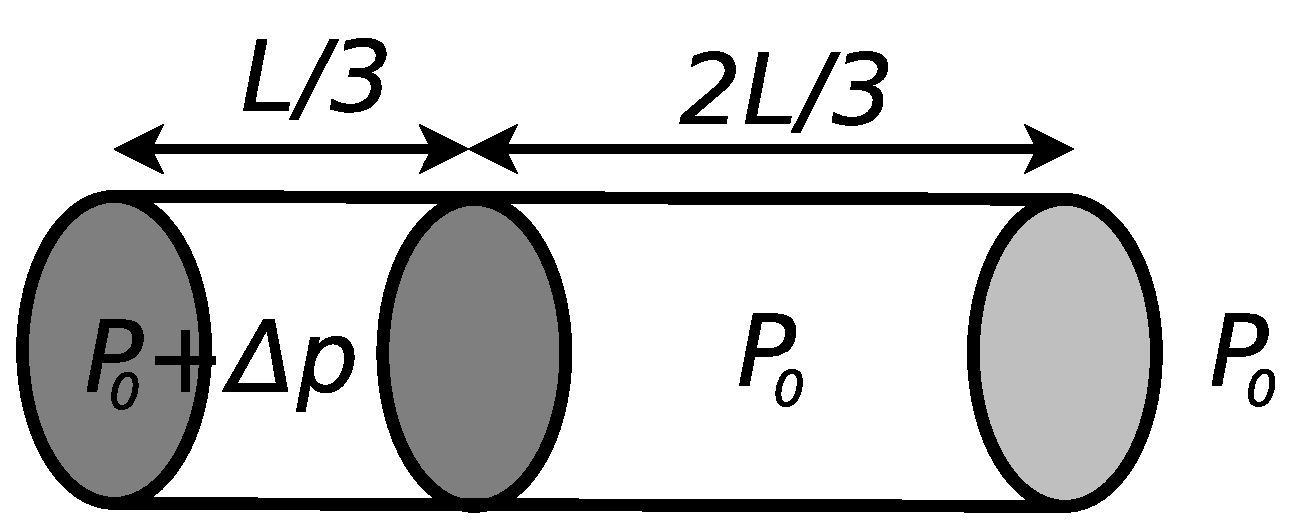
\includegraphics[width=\textwidth]{ej1-31}
\end{minipage}


